\section{The Dividend Problem}

The notion of the problem of dividends is popularized by De Fenetti (\cite{deF}) and starts by considering a Cramer-Lundberg process $\{ X(t) \}_{t \in [0,\infty] }$ (we can of course consider more general cases) and another process $\{ L(t) \}_{t \in [0,\infty] }$ which is left continuous, nonnegative, and non decreasing.\\
\bigskip
The quantity $L(t)$ can be thought of as the cumulative dividends paid up to time $t$ of an insurance company and hence the risk process taking into account the dividends is $\{ U(t) \}_{t \in [0,\infty] }$ where
\[
U(t) = X(t) - L(t).
\]
The general problem is the characterization of $L$ and the maximization of $U$ through the choice of $L$, often called a dividend strategy.

A dividend strategy is called admissible if at any time before ruin, all dividend payments are smaller than the current value of $U$, that is
\[L(t^+) - L(t) \leq U(t), \quad \forall t < \tau\]
where $\tau$ is the ruin time of $U$.\\
\bigskip
There are a number of possible dividend strategies, hence one often associates another parameter to the process $L$, say $L^{\pi}$.

Denoting all admissible strategies by $\Pi$, we write the expected value at the discount rate $q\geq 0$ associated with the dividend strategy $\pi \in \Pi$ with initial surplus $x \geq 0$ as
\[
V^{\pi}(x) = \mbbE_x \lt[ \int_0^{\tau^{\pi}} e^{-qt} dL^{\pi}_t \rt].
\]
One may sometimes see $V^{\pi}$ being referred to as the value function associated with strategy $\pi$. The problem is the characterization of
\[
V(x) = \sup_{\pi \in \Pi} V^{\pi}(x).
\]

Under the barrier strategy studied by Avram (\cite{APP}), the  process $U$ is never allowed to go above a constant level $b>0$, by setting
\[ L(t) = (X(t)-a)^+ = \max \{0, X(t)-a\}. \]
That is, surplus above the barrier $b$ is always paid as dividend.

\begin{figure}
\begin{center}
\caption{Sample path for a risk process and under a dividend barrier $b$}
    \begin{subfigure}[b]{0.3\textwidth}
        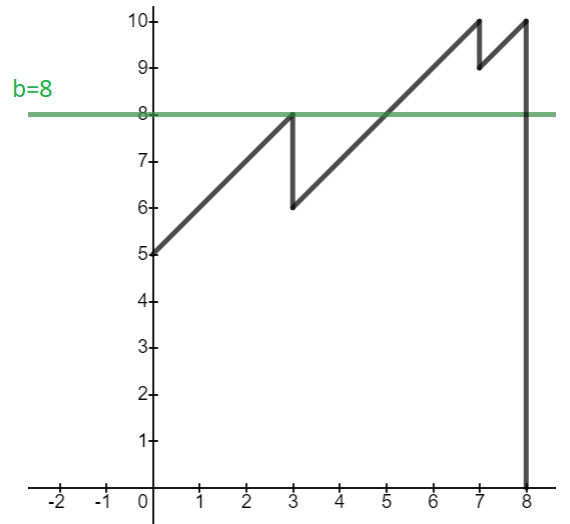
\includegraphics [width=2.2in]{divi1-1.png}
        \caption{$X(t)$}
        \label{fig:gull}
    \end{subfigure}\\
    \begin{subfigure}[b]{0.3\textwidth}
        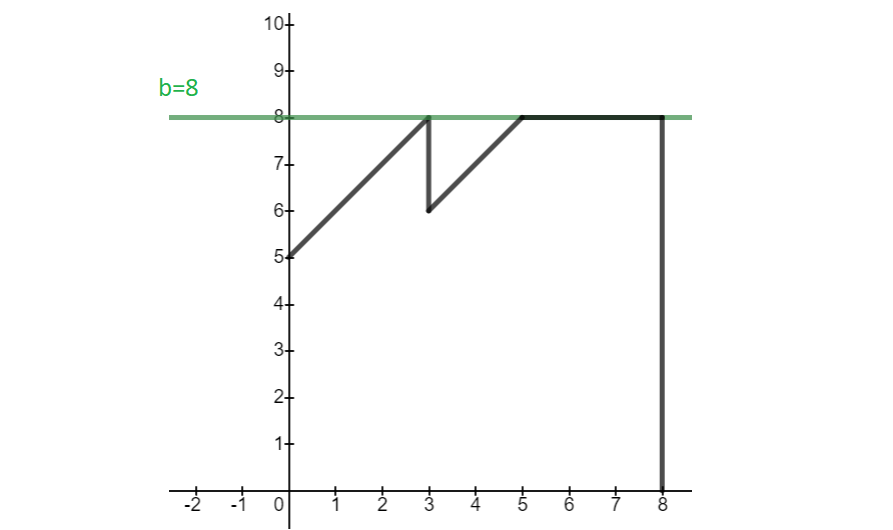
\includegraphics [width=3.3in]{divi2-1.png}
        \caption{$U(t)$}
        \label{fig:tiger}
    \end{subfigure}
\end{center}
\end{figure}

Clearly, this strategy, which we denote by $b] \in \Pi$, is admissible, and referencing Avram (2007), we have the following result.
\begin{thm}
Let $W_q$ be the associated scale function to $X$ under the discount rate $q\geq 0$. Under a constant dividend barrier strategy $b] \in \Pi$,
\[ V^{b]} (x) = \begin{cases}
\frac{W_q(x)}{W'_q(b)} & \text{ if $x \leq b$}\\
x - b + \frac{W_q(b)}{W'_q(b)} & \text{ if $x > b$}
\end{cases}
\]
\end{thm}

Looking at $V^{b]}$ as a function of $b$ instead of $x$, we can solve for $V$ by looking at where the derivative of $V^{b]}$ is zero. We summarize this result through the use of the `barrier function' $H$.
\begin{rmk}[\cite{APP}, \cite{Loef08}]
Let $b \geq 0$ and $H(b) = \frac{1}{W'_q (b)}$.\\
If $H$ is differentiable with $H'(0) > 0$, and has a unique local maximum $b^*>0$, then this $b^*$ yields the optimal barrier strategy, i.e. $V= V^{b^*]}$.\\
Furthermore, note that
\begin{itemize}
\item $H'(0) > 0 \iff W_q''(0)<0$
\item local maximum at $b^* \Rightarrow W_q''(b^*) =0$
\item uniqueness of local maximum at $b^* \Rightarrow H(b_1) \geq H(b_2)$, whenever $b* \leq b_1 \leq b_2$
\end{itemize}
\end{rmk}

This remark tells us that not only is $V^{b^*]}$ the optimal strategy over the space of the constant barrier strategies, but it is optimal over all strategies in $\Pi$.\\
\bigskip
We will not be tackling other dividend strategies in this presentation, nonetheless, we stress the fact that they do exist (see for example threshold strategies (\cite{gerber2004optimal}), multiband strategies (\cite{AM05}), etc.)

\subsection{The Cramer-Lundberg model with exponential jumps}
\label{CLexpo}

Consider the Cramer-Lundberg model $ X(t) = u + ct - S(t), \quad S(t) = \sum_{i=1}^{N_\lambda (t)} C_i $\\
where $C_i$'s are exponentially distributed with $\mbbE C_i = \frac{1}{\mu}$.\\
\bigskip
Standard computations yield
\[
\kappa(s)= s \lt( c- \frac{\lambda}{s + \mu} \rt), \quad \kappa'(0) = c - \frac{\lambda}{\mu}
\]
and solving
\[
\kappa(s)-q = 0 \iff cs^2 + (c\mu -\lambda -q ) s -q\mu = 0
\]
yields two distinct solutions $\gamma_1 \leq 0 \leq \gamma_2$ given by
\[
\gamma_1 = \frac{1}{2c} \lt( -(c\mu -\lambda -q ) + \sqrt{ (c\mu -\lambda -q )^2 + 4 c q\mu} \rt)
\]
\[
\gamma_1 = \frac{1}{2c} \lt( -(c\mu -\lambda -q ) - \sqrt{ (c\mu -\lambda -q )^2 + 4 c q\mu} \rt)
\]

In this example the Laplace transform of the $W_q$ scale function is
\[
\hat{W}_q(s) = \frac{1}{\kappa(s)-q} = \frac{s + \mu}{cs^2 + (c\mu -\lambda -q ) s -q\mu}
\]
which, when inverted becomes
\[
W_q(x) = \frac{(\gamma_1 + \mu)e^{\gamma_1 x} - (\gamma_2 + \mu) e^{\gamma_2 x} }{c(\gamma_1 - \gamma_2)}
\]

Differentiating we get
\[
W'_q(x) = \frac{\gamma_1(\gamma_1 + \mu)e^{\gamma_1 x} - \gamma_2(\gamma_2 + \mu) e^{\gamma_2 x} }{c(\gamma_1 - \gamma_2)}
\]
\[
W''_q(x) = \frac{\gamma_1^2(\gamma_1 + \mu)e^{\gamma_1 x} - \gamma_2^2(\gamma_2 + \mu) e^{\gamma_2 x} }{c(\gamma_1 - \gamma_2)}
\]
which implies
\[
W''_q(x) =0 \iff x = \frac{1}{\gamma_1 - \gamma_2} \log \frac{\gamma_2 (\gamma_2 + \mu)}{\gamma_1 (\gamma_1 + \mu)}.
\]

The function $W_q'(x)$ is unimodal with extremum at $x* = \frac{1}{\gamma_1 - \gamma_2} \log \frac{\gamma_2 (\gamma_2 + \mu)}{\gamma_1 (\gamma_1 + \mu)}$. Hence if
\[
W''_q(0)<0 \Rightarrow x* \text{ is a global minimum}
\]
and
\[
W''_q(0)\geq 0 \Rightarrow x* \text{ is a global maximum}.
\]
Therefore the optimal boundary $b*$ for the dividend problem is
\[
b*=
\begin{cases}
\frac{1}{\gamma_1 - \gamma_2} \log \frac{\gamma_2 (\gamma_2 + \mu)}{\gamma_1 (\gamma_1 + \mu)} & \text{ if } W''_q(0)<0\\
0 & \text{ if } W''_q(0)\geq 0.
\end{cases}
\]